\documentclass[11pt, a4paper]{article}
\usepackage{pdfpages}
\usepackage{parallel}
\usepackage[T2A]{fontenc}
\usepackage{ucs}
\usepackage[utf8x]{inputenc}
\usepackage[polish,english,russian]{babel}
\usepackage{hyperref}
\usepackage{rotating}
\usepackage[inner=2cm,top=1.8cm,outer=2cm,bottom=2.3cm,nohead]{geometry}
\usepackage{listings}
\usepackage{graphicx}
\usepackage{wrapfig}
\usepackage{longtable}
\usepackage{indentfirst}
\usepackage{array}
\usepackage{tikzsymbols}
\usepackage{soul}
\usepackage[ruled,vlined]{algorithm2e}
%\counterwithout{figure}{section} 

\usepackage{url}
\makeatletter
\g@addto@macro{\UrlBreaks}{\UrlOrds}
\makeatother

\newcolumntype{P}[1]{>{\raggedright\arraybackslash}p{#1}}
\frenchspacing
\usepackage{fixltx2e} %text sub- and superscripts
\usepackage{icomma} % коскі ў матэматычным рэжыме
\PreloadUnicodePage{4}

\newcommand{\longpage}{\enlargethispage{\baselineskip}}
\newcommand{\shortpage}{\enlargethispage{-\baselineskip}}

\def\switchlang#1{\expandafter\csname switchlang#1\endcsname}
\def\switchlangbe{
\let\saverefname=\refname%
\def\refname{Літаратура}%
\def\figurename{Іл.}%
}
\def\switchlangen{
\let\saverefname=\refname%
\def\refname{References}%
\def\figurename{Fig.}%
}
\def\switchlangru{
\let\saverefname=\refname%
\let\savefigurename=\figurename%
\def\refname{Литература}%
\def\figurename{Рис.}%
}

\hyphenation{admi-ni-stra-tive}
\hyphenation{ex-pe-ri-ence}
\hyphenation{fle-xi-bi-li-ty}
\hyphenation{Py-thon}
\hyphenation{ma-the-ma-ti-cal}
\hyphenation{re-ported}
\hyphenation{imp-le-menta-tions}
\hyphenation{pro-vides}
\hyphenation{en-gi-neering}
\hyphenation{com-pa-ti-bi-li-ty}
\hyphenation{im-pos-sible}
\hyphenation{desk-top}
\hyphenation{elec-tro-nic}
\hyphenation{com-pa-ny}
\hyphenation{de-ve-lop-ment}
\hyphenation{de-ve-loping}
\hyphenation{de-ve-lop}
\hyphenation{da-ta-ba-se}
\hyphenation{plat-forms}
\hyphenation{or-ga-ni-za-tion}
\hyphenation{pro-gramming}
\hyphenation{in-stru-ments}
\hyphenation{Li-nux}
\hyphenation{sour-ce}
\hyphenation{en-vi-ron-ment}
\hyphenation{Te-le-pathy}
\hyphenation{Li-nux-ov-ka}
\hyphenation{Open-BSD}
\hyphenation{Free-BSD}
\hyphenation{men-ti-on-ed}
\hyphenation{app-li-ca-tion}

\def\progref!#1!{\texttt{#1}}
\renewcommand{\arraystretch}{2} %Іначай формулы ў матрыцы зліпаюцца з лініямі
\usepackage{array}

\def\interview #1 (#2), #3, #4, #5\par{

\section[#1, #3, #4]{#1 -- #3, #4}
\def\qname{LVEE}
\def\aname{#1}
\def\q ##1\par{{\noindent \bf \qname: ##1 }\par}
\def\a{{\noindent \bf \aname: } \def\qname{L}\def\aname{#2}}
}

\def\interview* #1 (#2), #3, #4, #5\par{

\section*{#1\\{\small\rm #3, #4. #5}}
\ifx\ParallelWhichBox\undefined%
    \addcontentsline{toc}{section}{#1, #3, #4}%
\else%
\ifnum\ParallelWhichBox=0%
    \addcontentsline{toc}{section}{#1, #3, #4}%
\fi\fi%

\def\qname{LVEE}
\def\aname{#1}
\def\q ##1\par{{\noindent \bf \qname: ##1 }\par}
\def\a{{\noindent \bf \aname: } \def\qname{L}\def\aname{#2}}
}

\newcommand{\interviewfooter}[1]{
\vskip 1em
\noindent \textit{#1}
}

\switchlang{en}
\begin{document}

\title{1992 "--- Lotus Mouse}
\date{}
\maketitle
\selectlanguage{english}
The Lotus Mouse is a typical example of an optomechanical mouse from the 90s. The appearance of this mouse can be seen in figure \ref{fig:LotusPic}.

\begin{figure}[h]
    \centering
    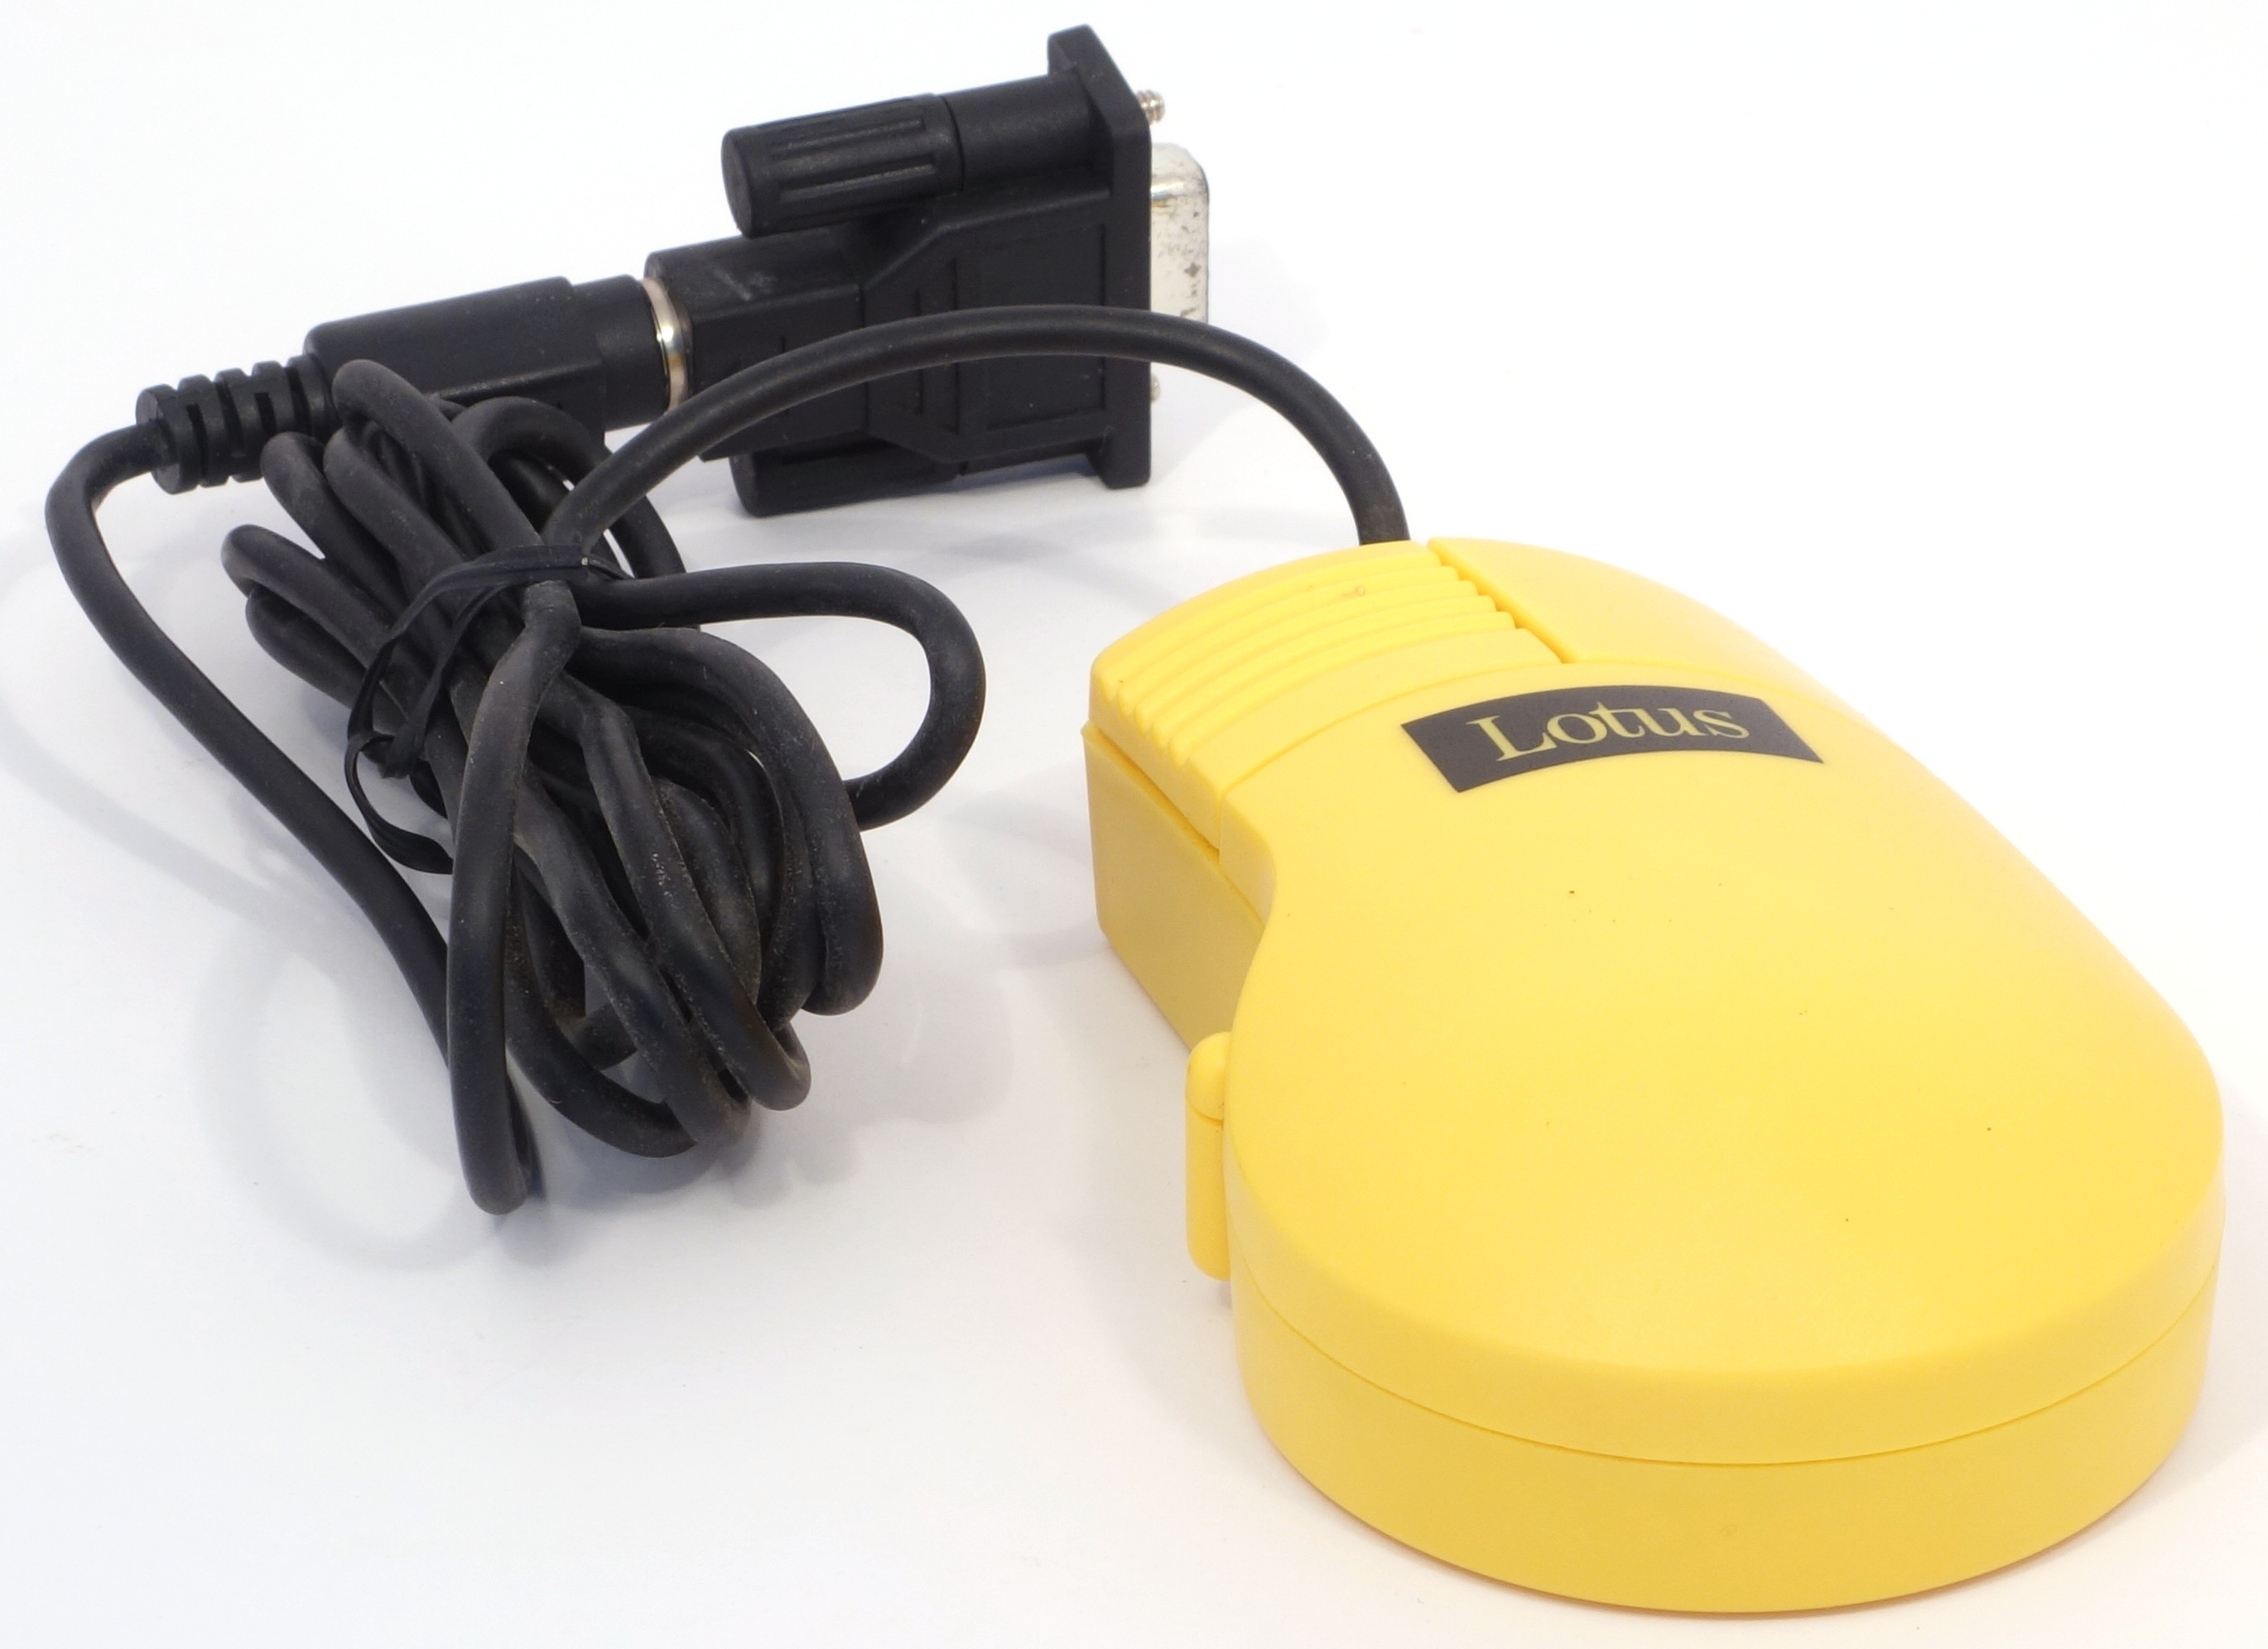
\includegraphics[scale=0.6]{1992_lotus_mouse/pic_30.jpg}
    \caption{Lotus Mouse}
    \label{fig:LotusPic}
\end{figure}

The mouse has an ergonomically shaped asymmetrical body and is designed for right-handed use (fig. \ref{fig:LotusHand}). On the upper side of the case there are two large buttons and the word “Lotus” is written. The surface of the main mouse button is embossed to make it easier to tactilely identify.

\begin{figure}[h]
    \centering
    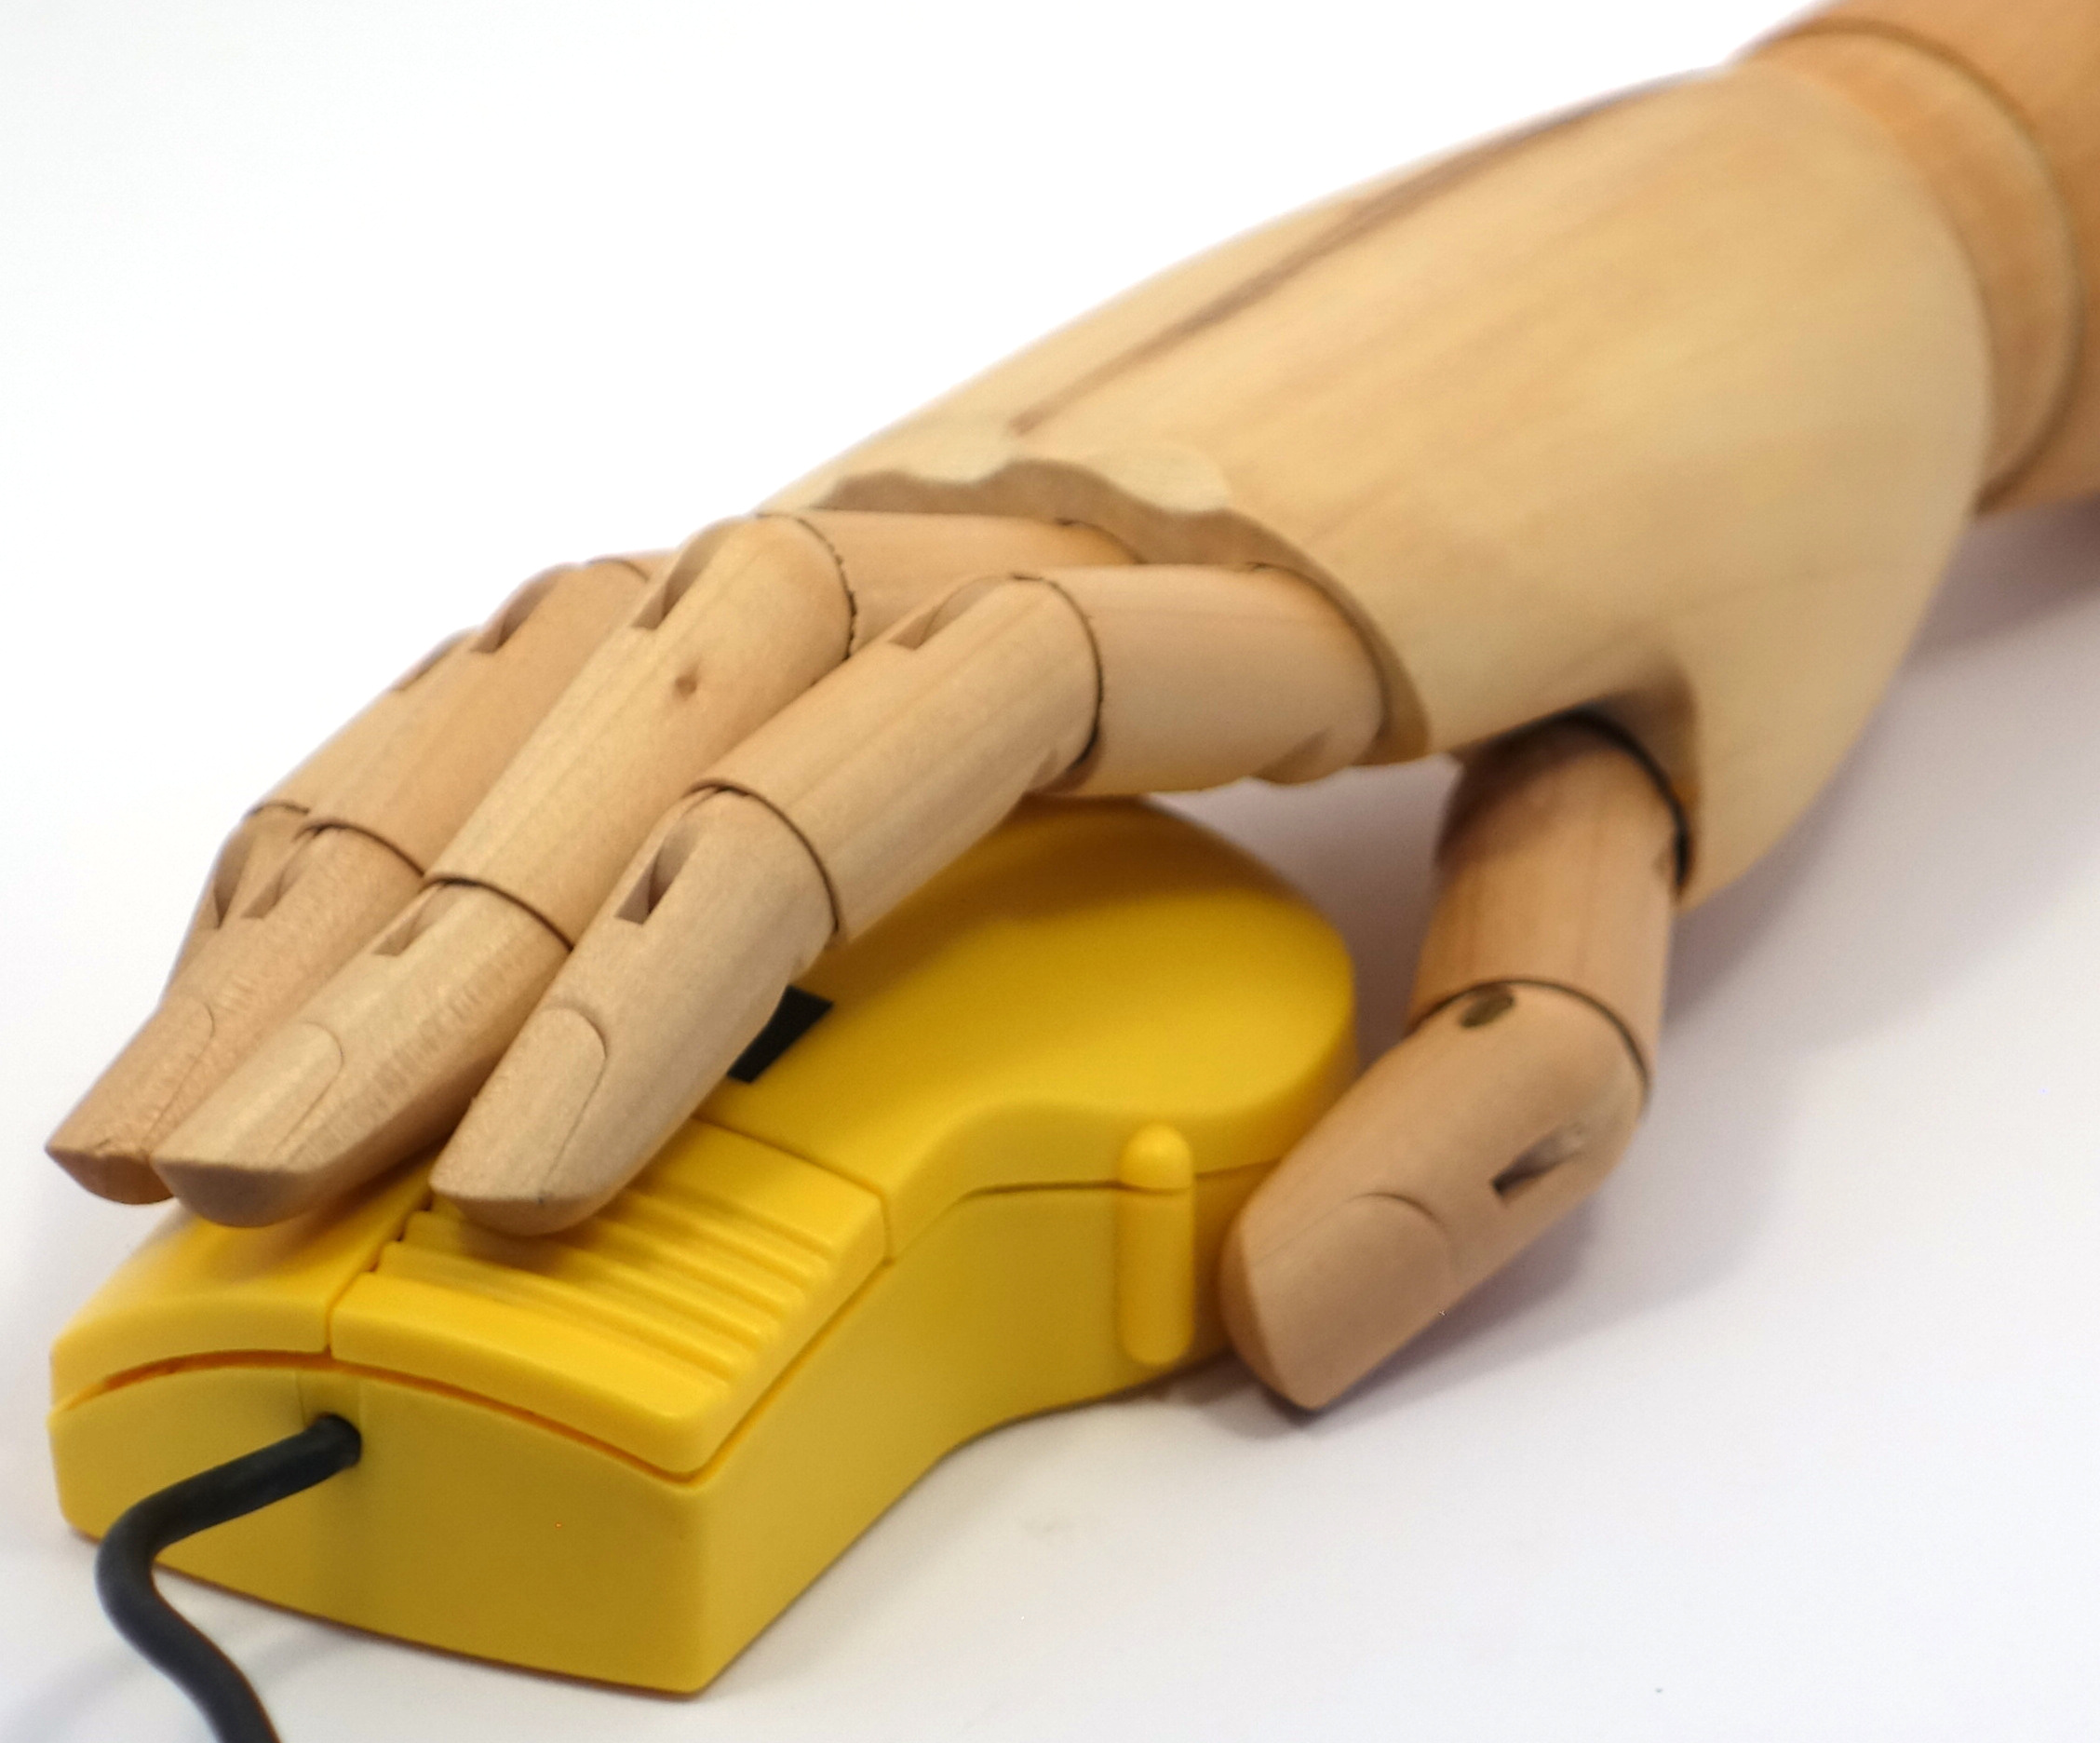
\includegraphics[scale=0.3]{1992_lotus_mouse/hand_30.jpg}
    \caption{Lotus Mouse with a human hand model}
    \label{fig:LotusHand}
\end{figure}

\begin{figure}[h]
    \centering
    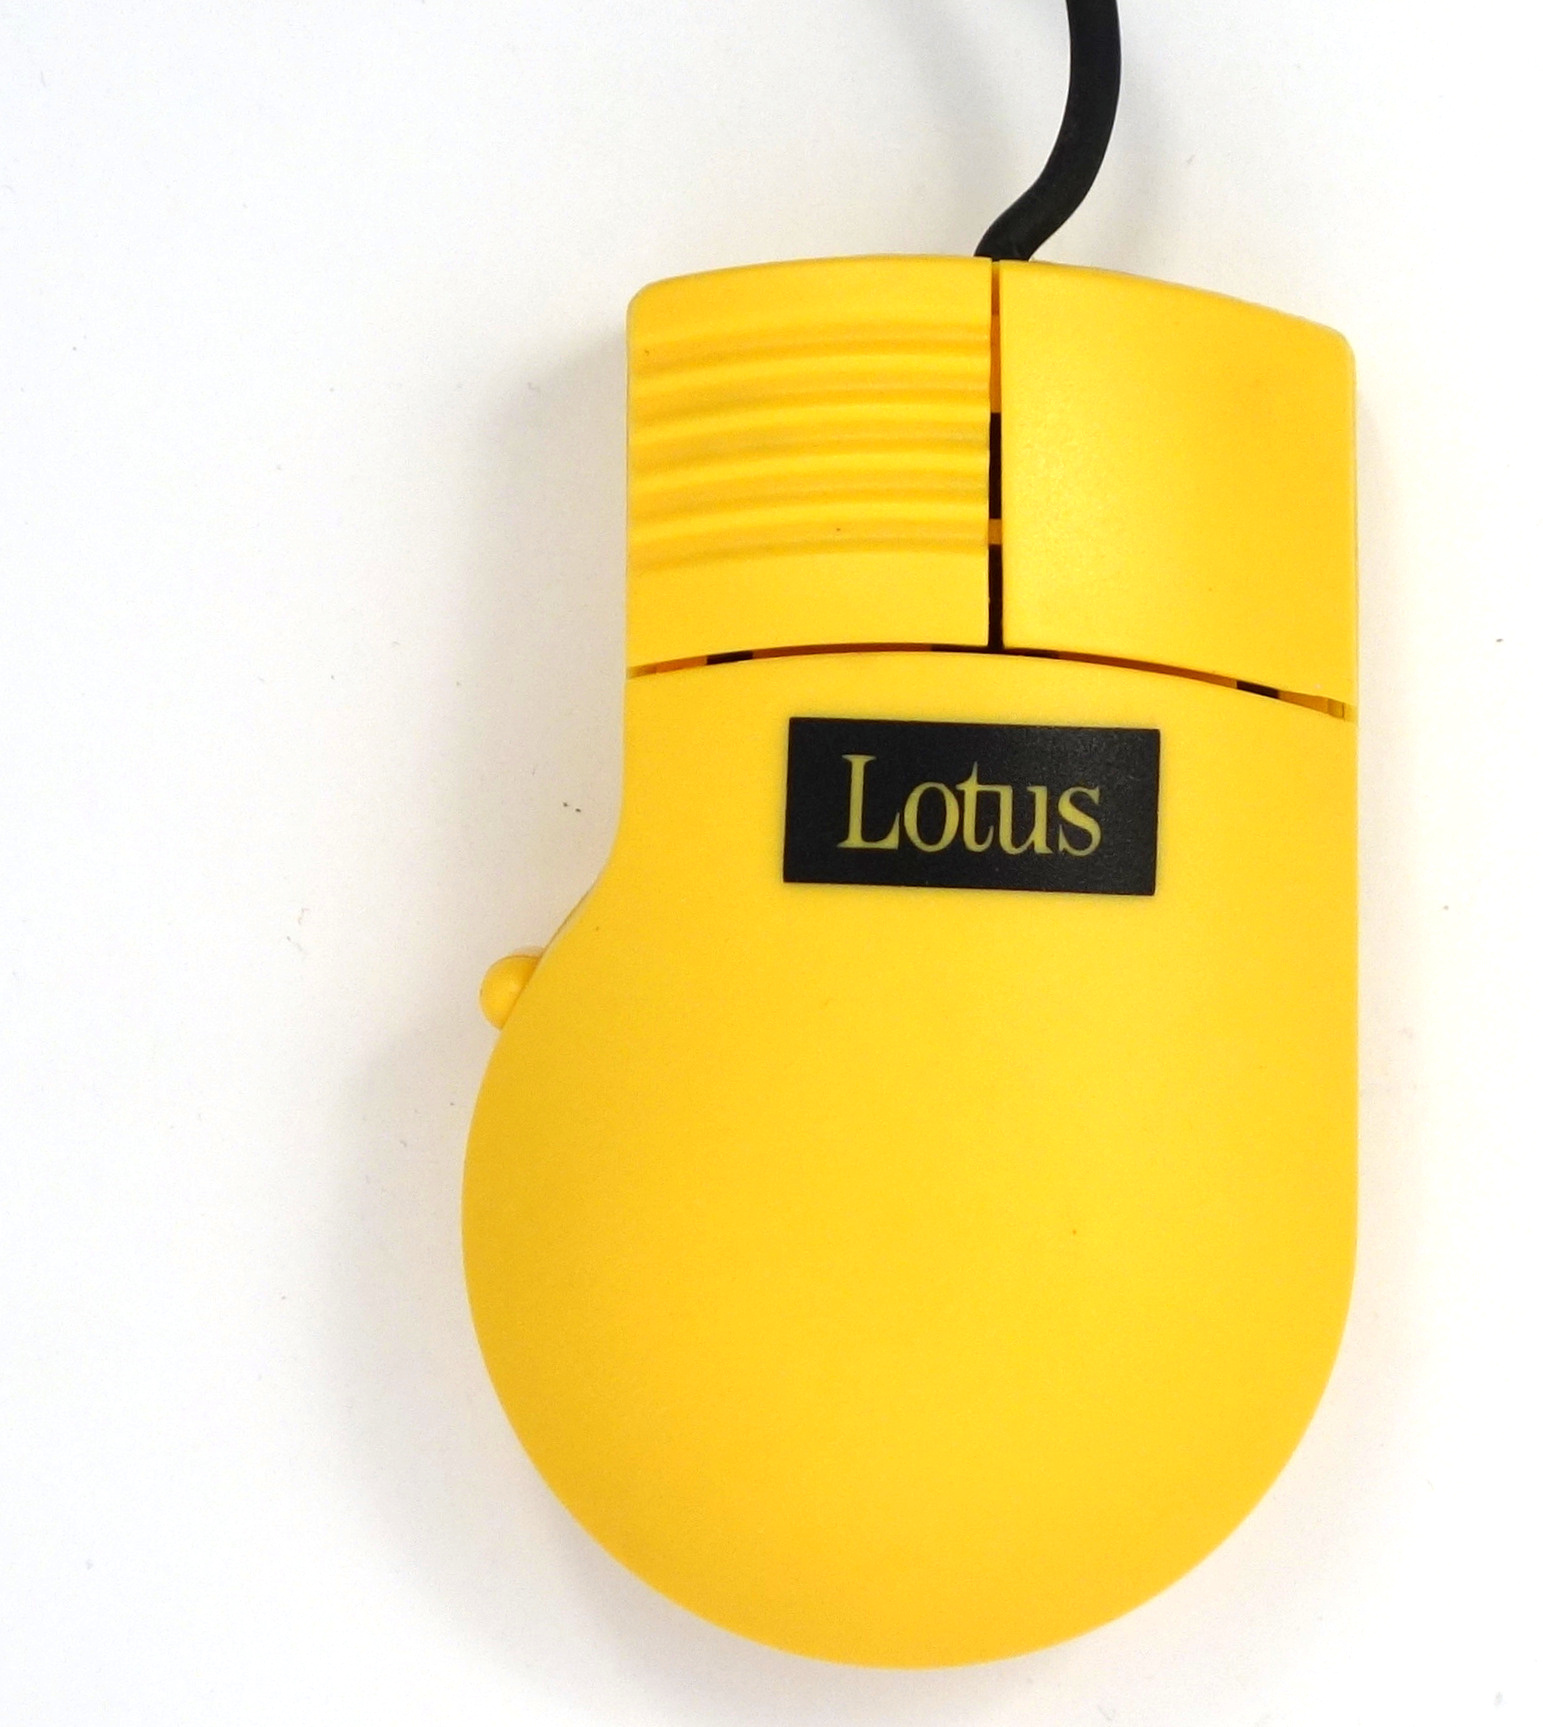
\includegraphics[scale=0.3]{1992_lotus_mouse/top_30.jpg}
    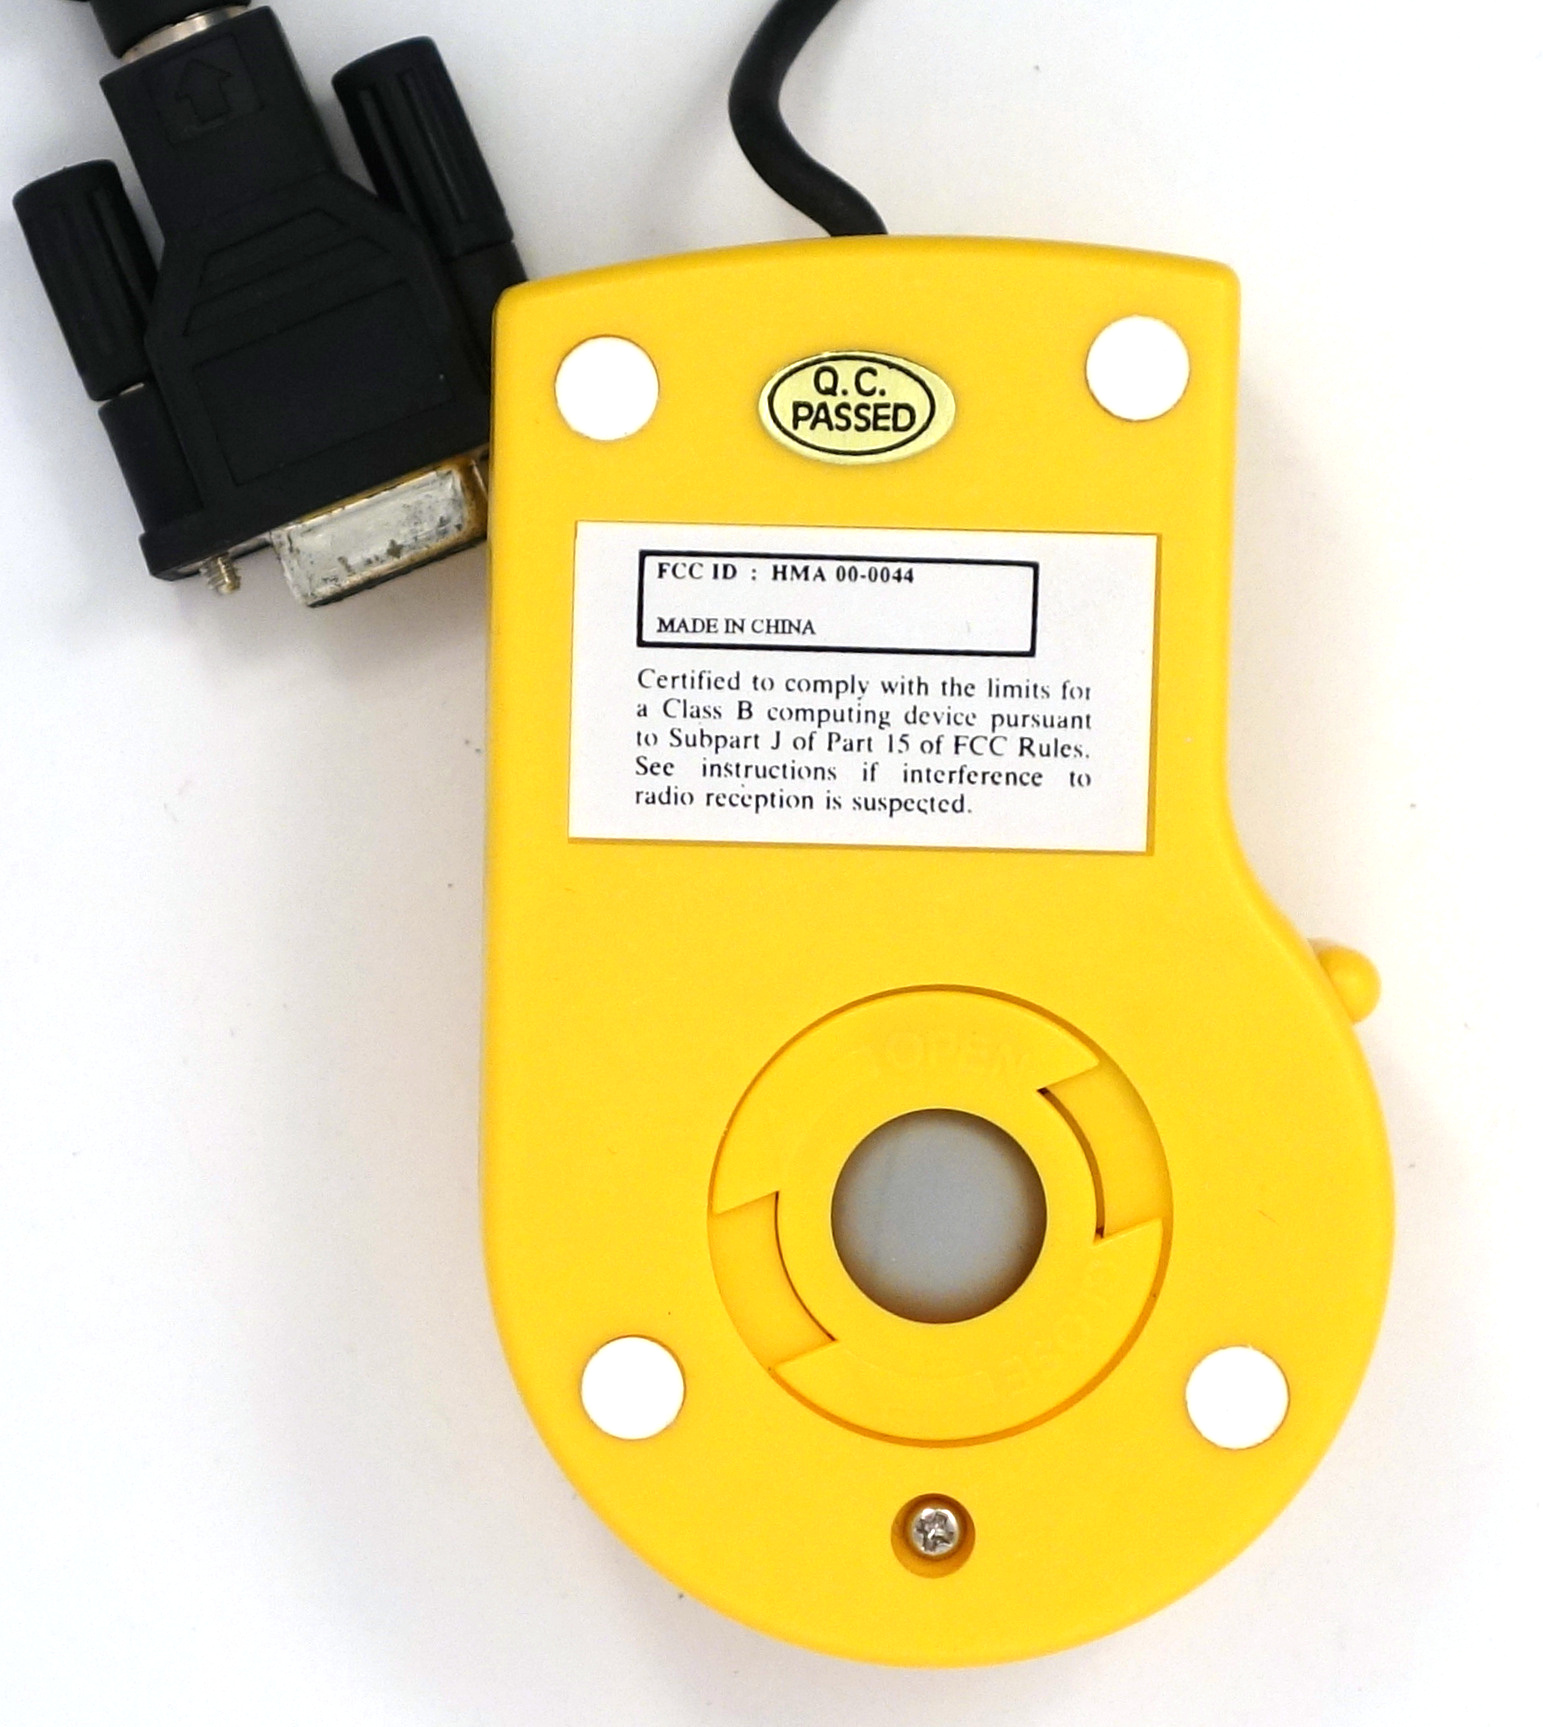
\includegraphics[scale=0.3]{1992_lotus_mouse/bottom_30.jpg}
    \caption{Lotus Mouse, top and bottom views}
    \label{fig:LotusTopBottom}
\end{figure}

Turning the mouse over (figure \ref{fig:LotusTopBottom}) reveals a rubber ball and low-friction polymer gliding feet.

The mouse is connected to the computer via a serial port.

\begin{figure}[h]
    \centering
    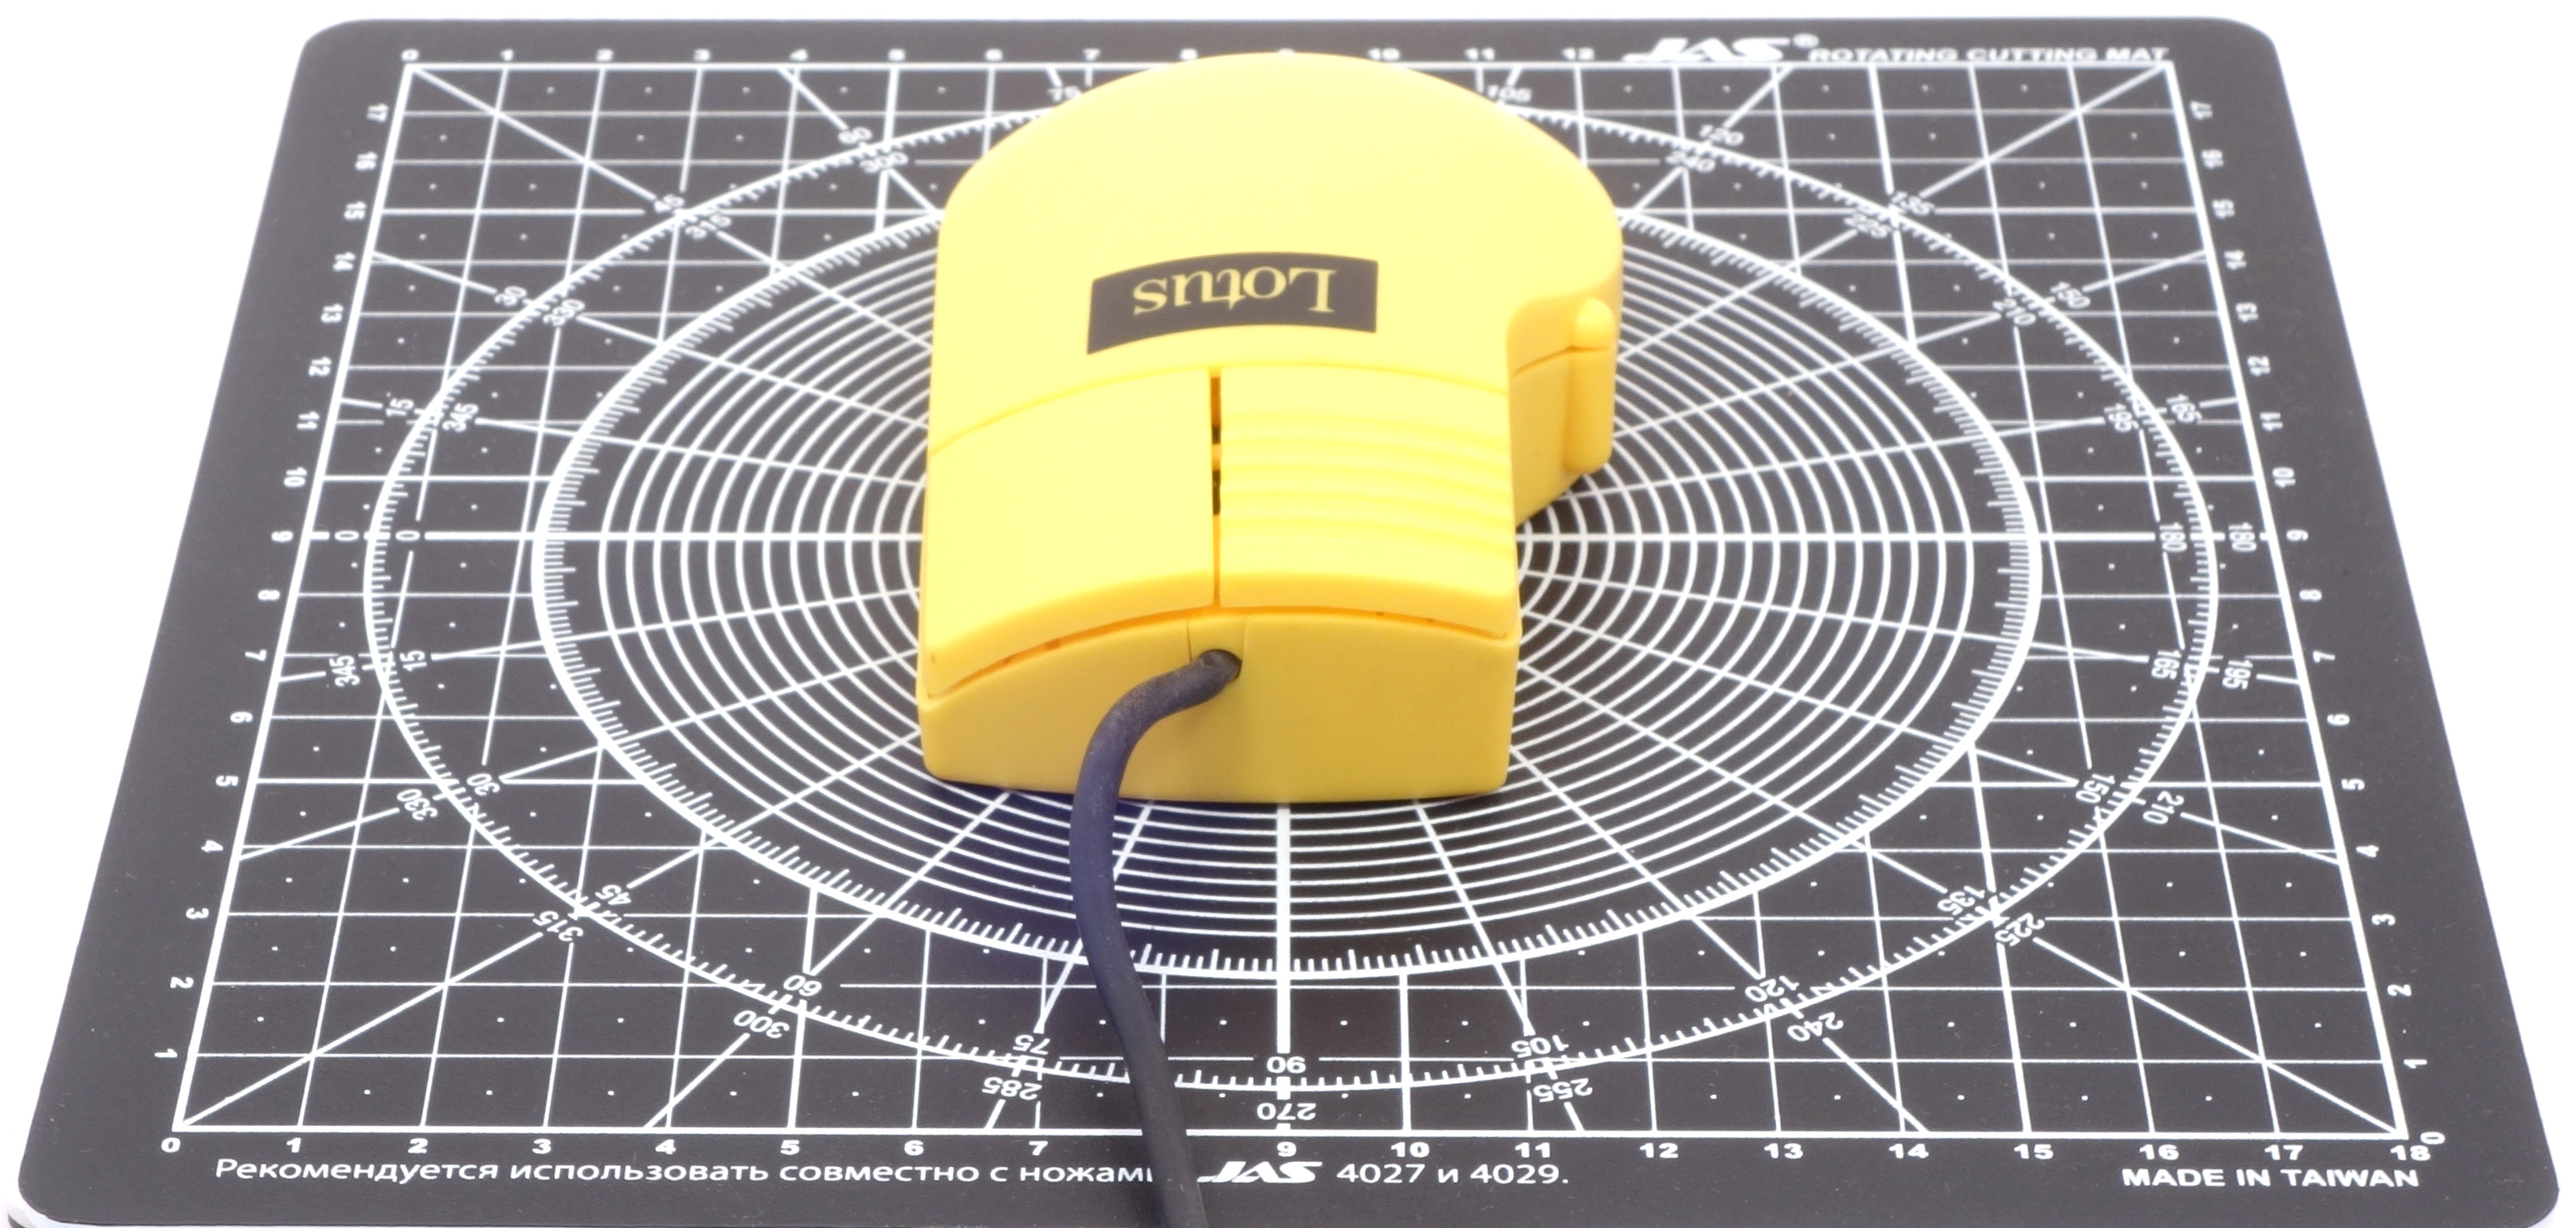
\includegraphics[scale=0.3]{1992_lotus_mouse/size_30.jpg}
    \caption{Lotus Mouse on a graduated pad with a grid step of 1~cm}
    \label{fig:LotusSize}
\end{figure}

It can be said that the Lotus Mouse is a forerunner of the Microsoft Mouse 2.0 shape to a certain extent - a mouse that was released a year later and then in its turn gave shape to Microsoft's most famous mouse, the IntelliMouse.

Mouse internals are shown on figure. \ref{fig:LotusInside}. It is a typical opto-mechanical device. The FCC ID code reveals that this mouse was manufactured in 1992 by the Taiwanese BMC Micro Industries company at the factory in Singapore.

\begin{figure}[h]
    \centering
    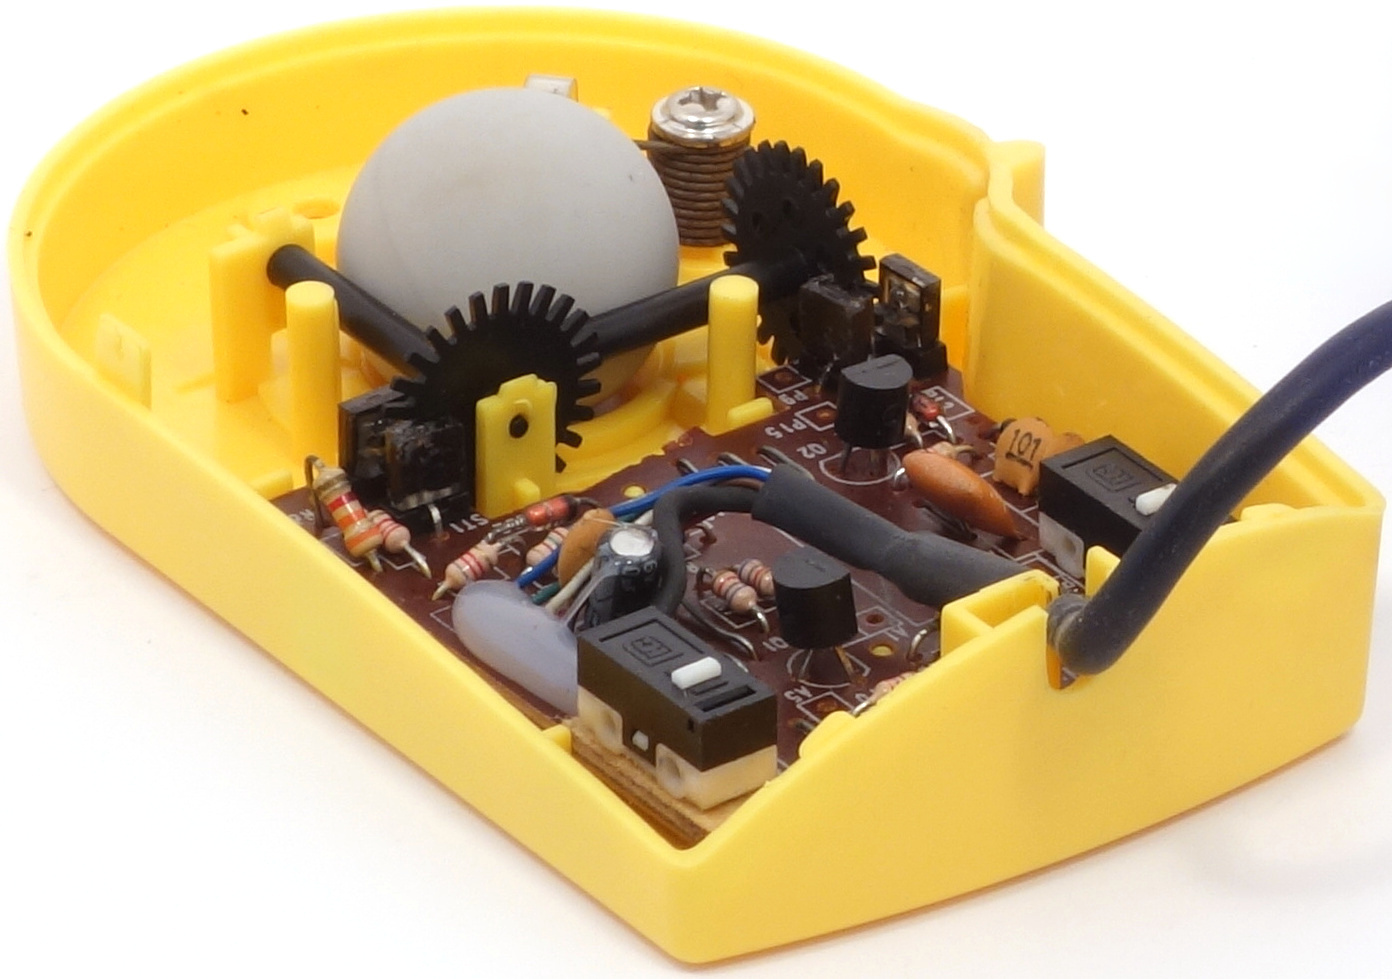
\includegraphics[scale=0.7]{1992_lotus_mouse/inside_30.jpg}
    \caption{Lotus Mouse disassembled}
    \label{fig:LotusInside}
\end{figure}



\end{document}
